\begin{figure}[h]
	\caption{\textbf{The CES exponent ($\rho$) as a function of the substitution elasticity}}
	\label{fig:CESFig}
	\centering

\pgfplotsset{every tick label/.append style={font=\scriptsize}}
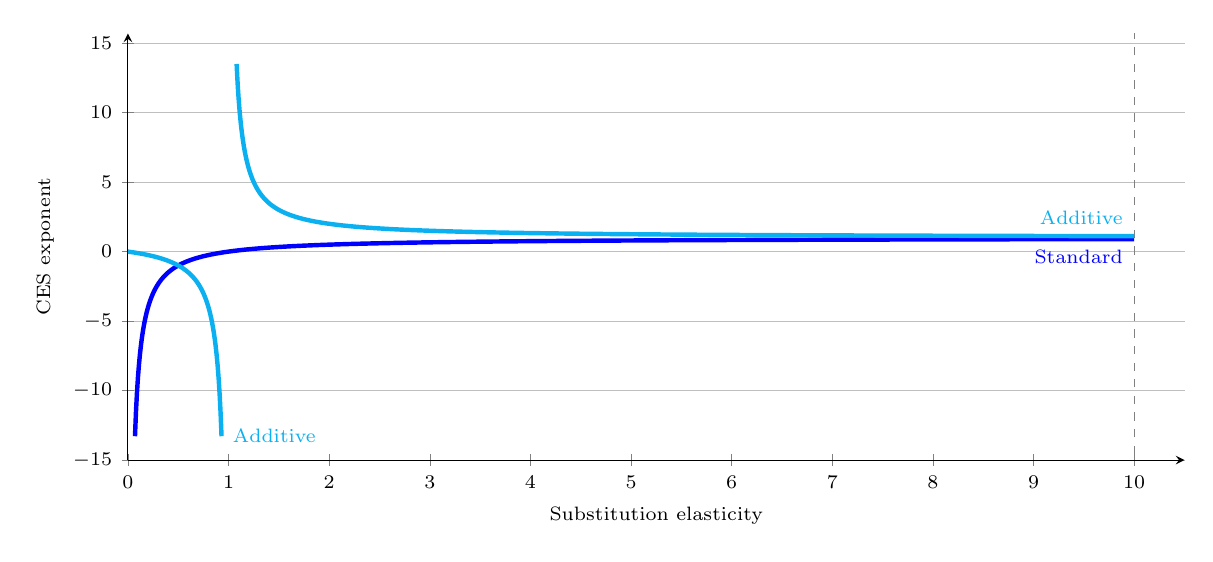
\begin{tikzpicture}
\begin{axis}[axis lines=left,xtick={0,1.0,...,10.0},xmin=0,xmax=10.5,
						     ytick={-15,-10,...,15},ymin=-15.0,ymax=15.7,
						     width=15cm,height=7cm,
x tick label style={
	/pgf/number format/.cd,
	fixed,
	fixed zerofill,
	precision=0,
	ymajorgrids,
	xlabel={\scriptsize{Substitution elasticity}},
	ylabel={\scriptsize{CES exponent}},
	/tikz/.cd
}]

\draw[dashed,color=gray] (10,-600) -- (10,600) ;

\addplot[mark=none,blue,ultra thick,domain=0.07:10,samples=1000]{(x-1)/x} node[below left] {\scriptsize{Standard}} ;
\addplot[mark=none,ProcessBlue,ultra thick,domain=0:0.93,samples=100]{x/(x-1)} node[right] {\scriptsize{Additive}} ;
\addplot[smooth,mark=none,ProcessBlue,ultra thick,domain=1.08:10,samples=1000]{x/(x-1)} node[above left] {\scriptsize{Additive}} ;

\end{axis}
\end{tikzpicture}
\end{figure}
